\section{Qualitative Analysis}
\label{sec:qualitative}

The signed intersection changes in Fig.~\ref{fig:dev-cases} show how two writes of the same size can have different effects. On HRSID DEV705, the seed-5217 point head improved 1,012 of the 1,461 eligible RF-DETR matches when the fixed pairs were released. It degraded 252 and tied 197. The two illustrated cases were selected nearest the median continuous-IoU difference within each sign, with distinct images. Both policies add eight and remove eight cells. In Fig.~\ref{fig:dev-cases}(a), independent selection recovers one extra pixel-equivalent of polygon area through additions and retains another 1.5 through deletions. Continuous IoU rises from 80.63 to 81.36. In Fig.~\ref{fig:dev-cases}(b), the additions of both policies miss the reference. Independent selection then removes one more pixel-equivalent of covered hull, reducing IoU from 76.19 to 75.87. Predicted occupancy ranks the competing sites incorrectly in this case.

\begin{figure*}[!t]
\centering
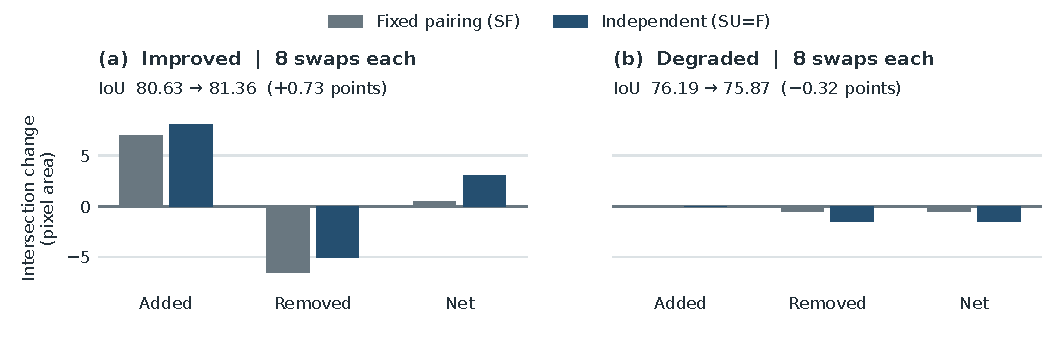
\includegraphics[width=0.83\textwidth]{figures/dev705_overlap_cases.pdf}
\caption{Observed RF-DETR matches on HRSID DEV705, occupancy-head seed 5217. Both policies use eight additions and eight removals. Bars show the reference intersection gained by additions, lost through deletions, and the net change from the native mask. The two cases are nearest the median of the observed IoU differences within each sign. All values use the native cells and the original polygon.}
\label{fig:dev-cases}
\end{figure*}

Fig.~\ref{fig:segrefiner-cases} gives a wider-edit comparison on Instance-RSDD. The published SegRefiner-LR writer~\cite{segrefiner} improves 14 of the 39 eligible reference matches it edits and worsens 25. In the median-sign improvement, the writer trims an extension beyond the hull and raises IoU from 58.68 to 60.96. In the loss case, the write removes reference area at both ends and along a narrow side, lowering IoU from 71.93 to 67.43. The local occupancy writes give 58.89 and 71.95 on these same references. The mixed outcomes are consistent with the signed-loss analysis below. The spatial pooling in the display can break a thin reference contour into segments. The overlap values use the unpooled masks.

\begin{figure*}[!t]
\centering
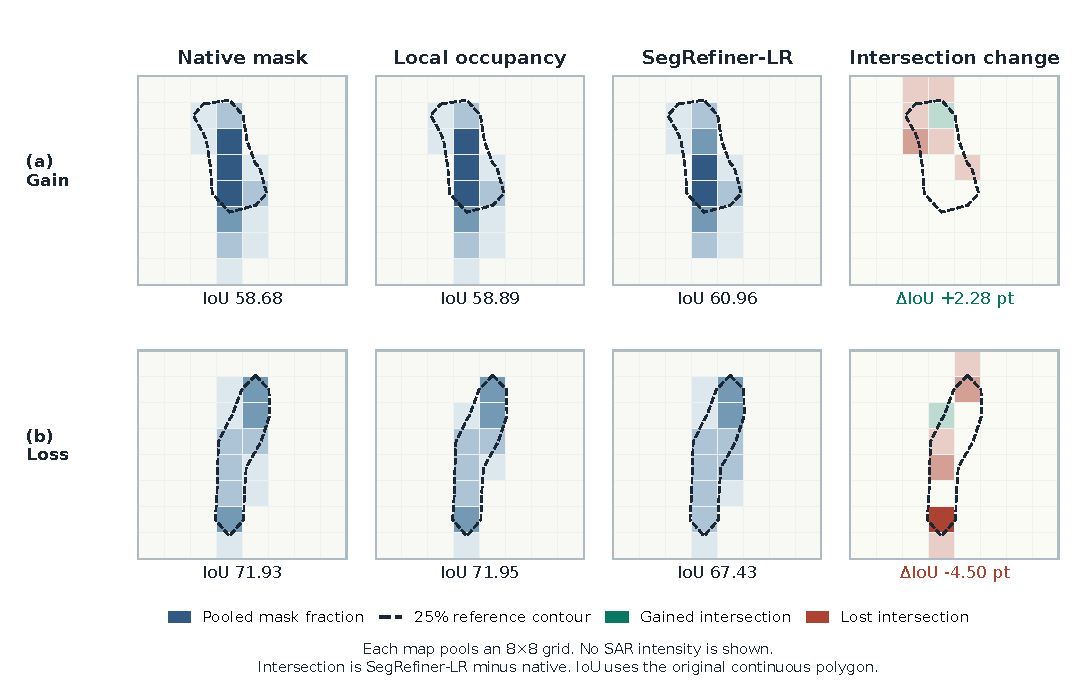
\includegraphics[width=0.87\textwidth]{figures/rsdd74_segrefiner_cases_binned.pdf}
\caption{Observed gain and loss from the original SegRefiner-LR writer on the Instance-RSDD reserve, with the native and local occupancy masks on the same matches. The cases are nearest the within-sign medians among 39 exposed matches. The public panels pool spatial occupancies and intersection changes into an \(8\times8\) grid and display the 25\% reference-occupancy contour. IoU and area changes use the original native raster and author polygon.}
\label{fig:segrefiner-cases}
\end{figure*}

\FloatBarrier
\section{Ablation Studies}
\label{sec:ablation}

\subsection{Independent addition and removal positions}

We combine the addition and removal sites from the fixed-pair and independent writes in a \(2\times2\) comparison. Each hybrid inherits its detector score, writable support, and realized signed counts from the same candidate. On the 74-chip reserve, each arm makes 30,841 exchanges across the complete stream. The factorial comparison therefore isolates the positions chosen on each side of the original mask.

\begin{table*}[t]
\centering
\caption{Mask AP in points for the spatial choice on each side at identical signed counts. Gaofen-3 uses two head fits on the same 583 chips and the same frozen detector. The 42-chip date-separated view is nested within the reserve.}
\label{tab:signed-side-ablation}
\footnotesize
\begin{tabular}{@{}llrrrr@{}}
\toprule
View & Head seed & Both fixed & Independent add & Independent remove & Both independent\\
\midrule
Gaofen-3, 583 chips & 5217 & 61.036 & 61.331 & 61.286 & \textbf{61.518}\\
Gaofen-3, 583 chips & 5218 & 60.984 & 61.207 & 61.302 & \textbf{61.468}\\
Reserve, 74 chips & 5217 & 58.278 & 58.545 & 58.426 & \textbf{58.714}\\
Date-separated, 42 chips & 5217 & 61.283 & 61.769 & 61.698 & \textbf{62.123}\\
\bottomrule
\end{tabular}
\end{table*}

Each single-side change raises mask AP, and freeing both sides gives the highest AP in all four rows of Table~\ref{tab:signed-side-ablation}. On Gaofen-3, independent selection on both sides gains 0.175 continuous-IoU points over independent additions alone (paired 95\% interval \([0.130,0.222]\)) and 0.085 over independent removals alone (\([0.049,0.120]\)). The corresponding gains on the reserve are 0.170 (\([0.108,0.251]\)) and 0.148 (\([0.042,0.252]\)) across 47 eligible matches in 12 parents. The two signed changes are additive in intersection area at a fixed hull. The AP interaction ranges from \(-0.063\) to \(+0.020\) points across the main views, where edited masks can alter matching at each threshold.

\subsection{Ranking, support, and the number of writes}

A geometric ranking remains competitive under the same spatial and count constraints. On the 74-chip reserve, occupancy ranking at the dynamic-attraction budget~\cite{atkinson} gains 0.468 AP and 0.431 continuous-IoU points over dynamic attraction, and 0.203 AP and 0.301 IoU over static attraction. Static attraction leads by 0.173 AP75. Capped PointRend~\cite{pointrend} supplies a learned control on the same endpoints and counts. On Gaofen-3, occupancy improves on it by 0.312 AP and 0.250 fixed-match IoU points. Full RoI PointRend has 0.200 higher AP than the complete-support occupancy writer and 1.744 lower AR100. The full paste changes support and edit counts. These comparisons separate ranking quality from the performance of the complete refinement pipeline.

We also cross the writable support and the flip limit on the same frozen five-iteration Phoenix response~\cite{phoenix}. On the PSeg-SSDD official allocation, imposing the exact count on the whole grid reduces writes from 3,391,327 to 147,540. This raises AP by 2.525 points and fixed-match IoU by 4.001 points (\([2.644,5.382]\)). Applying the count limit on sampled support raises IoU by 0.422 points, so the strongest effect of the limit occurs when the whole grid is writable. Within sampled support, equal signed counts then add 1.842 AP and 1.151 IoU points over the free split at exactly 147,540 flips. Static attraction still leads the balanced Phoenix writer by 0.195 AP at that budget. On the 74-chip reserve, the author LVIS whole-mask policy loses 17.779 AP points relative to same-response matched-count writing. The matched-endpoint Phoenix ranking itself leads occupancy by 0.308 AP, with a paired IoU interval spanning zero.

For SegRefiner-LR, applying the original deletions lowers continuous IoU by 4.092 points relative to native on the 39 exposed Instance-RSDD matches, and by 4.087 relative to retaining the original additions alone. The corresponding losses on 67 exposed PSeg-SSDD matches are 4.03 and 3.98 points. A deletion cap based on the number of additions recovers 0.907 and 0.878 AP points over the original writer. The capped policies trail the addition-only and local occupancy policies on these two evaluated cohorts. Preserving predicted area and preserving the useful part of a proposed update are distinct design choices.

\subsection{Spatial dependence in the allocation score}

We fit a joint model for disjoint four-neighbor endpoint pairs, motivated by the dependence studied in RankSEG-DEP~\cite{rankdep}. The models share endpoint marginals and the same finite signed action menus. Relative to independent predictions of the same pairs, the joint model lowers four-state Brier loss by 0.058 and 0.089 on held FIT groups under the two references. It also improves on coefficients fit after sign-preserving nonspatial rewiring. With frozen coefficients, spatially dependent expected-IoU selection alters 212 of 8,785 positive-budget candidate writes compared with independent expected-IoU selection. Only one of 206 common positive-budget native matches changes. Mask AP is identical under both references. Fixed-match raster IoU changes by zero and 0.00175 points, with the latter paired interval touching zero. This diagnostic supports a local probability-model improvement on the represented FIT groups and a small effect on the tested source decisions.

\section{Discussion and Reproducibility}
\label{sec:discussion}

The reference mask matters most where the editor changes the label. On the same 232 historical SSDD images, the natural-count endpoint policy gains 0.344 AP points over native under PSeg-SSDD and loses 0.491 under SPSD. Under variable signed allocation on SAR-SSP, the two frozen occupancy outputs are checked against the same author raster. Their signed intersection-gain overestimates are 0.896 and 0.628 points of reference area on the selected edits. For that contrast, 392 of the 393 gained false-foreground cells connect to the largest component containing retained fixed-policy foreground. The evidence places the excess chiefly on an attached region. These diagnostics concern selected mask changes under the available annotations.

Proposal coverage further bounds the utility of post-processing. In the frozen RF-DETR SAR-SSP comparison, reference-guided edits within the original support and cap recover just one of 47 unmatched hulls at mask IoU 0.50. Arbitrary replacement within the existing boxes admits nine recoveries at fixed area and a further 19 if area can vary. The latter figures are per-hull ceilings that permit reuse of a candidate. The small UEIKAP positive-budget population~\cite{ueikap} provides another case where few released hulls can benefit from editing. Geometry gains also have limited implications for physical sizing. Measured length-error changes in the common NovaSAR and Sentinel-1 AIS cohorts are uncertain under the paired intervals~\cite{nastar,gulf}.

The two Gaofen-3 detector fits share initialization and evaluation images. The 42-chip date-separated evaluation is nested within the Instance-RSDD reserve. These dependencies bound the transfer interpretation. For the prospective Umbra study, native, local, and Phoenix predictions are frozen on 12 preselected windows. A separate 24-acquisition supplement has completed native readback and frozen local-edit replay. Both await the two independent reference returns and scoring. Each has its own predeclared acquisition-coverage and interval criteria.

On the 74-chip reserve, with detector outputs available, mean single-thread refinement costs are 227.1 ms/image for occupancy writing, 1,221.5 for same-count PointRend, and 1,049.2 for full RoI PointRend. The same-count hybrid still renders the complete RoI. The \href{https://github.com/bingzhi495-creator/SAR-SEAL-research}{project repository} provides configuration, evaluation code, editable figures, and verified aggregate scores. Independent replay reproduced 3,434 tabulated entries on HRSID official and Instance-RSDD test and 1,470 entries on the 74-chip reserve with detector 5202 and head 5217. Exact reproduction requires the designated frozen weights, supplied separately, and the original annotations obtained through the documented dataset providers.
